%\documentclass[spanish,12pt,a4paper,titlepage,twoside,openright]{scrbook}
\documentclass[12pt,a4paper,titlepage]{report}
%\usepackage[latin1]{inputenc}
\usepackage[utf8]{inputenc}
\usepackage{graphicx}
\usepackage{subfig}
\usepackage{float}
\usepackage{wrapfig}
\usepackage{multirow}
\usepackage{caption}
\usepackage[spanish]{babel}
\usepackage[dvips]{hyperref}
\usepackage{amssymb}
\usepackage{listings}
\usepackage{epsfig}
\usepackage{amsmath}
\usepackage{array}
\usepackage[table]{xcolor}
\usepackage{multirow}
\usepackage{hhline}
\usepackage{cancel}

\usepackage[Sonny]{fncychap}
%\usepackage[Glenn]{fncychap}
%\usepackage[Conny]{fncychap}
%\usepackage[Rejne]{fncychap}
%\usepackage[Bjarne]{fncychap}

\usepackage{subfiles}
\usepackage{framed}
\usepackage{appendix}
\setlength{\topmargin}{-1.5cm}
\setlength{\textheight}{25cm}
\setlength{\oddsidemargin}{0.3cm} 
\setlength{\textwidth}{15cm}
\setlength{\columnsep}{0cm}
%\setkomafont{disposition}{\normalfont\bfseries}
\captionsetup{tablename=Tabla}

\ChNameVar{\bfseries\LARGE\sf}\ChNumVar{\fontsize{62}{65}\selectfont}
\ChTitleVar{\bfseries\LARGE\sf} \ChRuleWidth{2pt} \ChNameAsIs
\ChTitleAsIs
\renewcommand\FmN[4]{}
\newcommand{\HRule}{\rule{\linewidth}{0.5mm}}

\begin{document}


\begin{titlepage}
\begin{center}
\vfill
%\vspace{50cm}
\textsc{\LARGE Facultad de Ingenier\'ia de la Universidad de la Rep\'ublica}\\[1.5cm]
\vspace{2cm}
\textsc{\LARGE Procesamiento Digital de Señales de Audio\\[1cm]Curso 2012}\\[0.5cm]
\vspace{2.3cm}
% Title
\HRule \\[0.4cm]
{ \huge \bfseries Beat Tracking}\\[0.4cm]
\HRule \\[1.5cm]
\vspace{2cm}
% Author and supervisor
%\begin{center}
\begin{minipage}{0.4\textwidth}
\begin{flushleft} \large
\emph{Autores:}\\
%\begin{center}
%\begin{LARGE}
Gonzalo \textsc{Gutiérrez}\\ Mat\'ias \textsc{Tailani\'an}
%\end{LARGE}
%\end{center}
\end{flushleft}
\end{minipage}
%\end{center}
\begin{minipage}{0.4\textwidth}
\begin{flushright} \large
\end{flushright}
\end{minipage}

\vspace{2cm}

\vfill
\begin{figure} [h!]
\centering
\subfloat{
\includegraphics[width=0.25\textwidth]{./pics/logoIIE_transparente.png}}\hspace{1cm}
\subfloat{
\includegraphics[width=0.15\textwidth]{./pics/logo_fing_transparente.png}}\hspace{1cm}
\subfloat{
\includegraphics[width=0.15\textwidth]{./pics/logo_udelar.png}}
\end{figure}

% Bottom of the page
{\large \today}
\end{center}
\end{titlepage}



\chapter*{Introducción}
\vspace*{-1cm}
Al escuchar música una reacción inconsciente muy común es mover el pie golpeando el piso a tiempo con el \textbf{beat}. La tarea computacional que intenta replicar ese comportamiento es conocida como \textbf{beat tracking}.\\

La métrica de la señal se puede pensar como una estructura de pulsos percibidos a diferentes escalas temporales en una pieza musical. Se consideran 3 niveles métricos básicos: el \emph{tatum}, el \emph{tactus} o \emph{beat} y el \emph{compás}. El tatum es el valor en tiempo más pequeño que puede encontrarse en una pieza musical, es la unidad atómica de la pieza. En general los otros valores de duración presentes en la pieza son múltiplos de tatum. El tactus o beat está más relacionado con el aspecto semántico, y está directamente vinculado con el \textbf{tempo} de la pieza. Por último el compás está vinculado con la tasa de cambios armónicos o la duración de un patrón rítmico.\\

El problema del seguimiento de beat o \emph{beat tracking} es un problema todavía abierto, donde se sigue intentando con gran actividad lograr mejorar los resultados del estado del arte. Tiene un atractivo muy importante en sí mismo pensando en aplicaciones como el acompañamiento automático, asistencia a la hora del editado, estudios musicológicos, efectos de música adaptativos, o seguimiento del ritmo de una batería tocando en vivo, pero además es una parte imprescindible de algunos sistemas más complejos para aplicaciones como etiquetado de música, reconocimiento automático del género, análisis de similitud de música y para lograr la \emph{transcripción automática de música}.\\

El presente trabajo presenta un algoritmo de seguimiento de \emph{beat} de una pieza musical y se basa en el trabajo de ``Jo\~ao Lobato Oliveira, Fabien Gouyon, Luis Gustavo Martins, Luis Paulo Reis'', titulado ``IBT: A real time tempo and beat tracking system, presentado en la \emph{$11^a$ International Society for Music Information Retrieval Conference, ISMIR}, en 2010'' (\cite{bib:el_posta}). Dicho trabaja se basa a su vez en el sistema \textbf{BeatRoot}, presentado en (\cite{bib:dixon}): Dixon S., ``Automatic extraction of tempo and beat from expressive performances.'', \emph{Journal of New Music Research}, 2001. De \cite{bib:dixon} se toma la idea de varios \textbf{agentes} compitiendo y llevando varias hipótesis de tempo y fase paralelamente, se agrega robustez ante entradas ruidosas y se implementa en tiempo real. Aún realizando todas las operaciones de forma causal y en tiempo real, se logra obtener resultados comparables con el estado del arte y se convierte además en el primer software \emph{open source} de seguimiento de beat en tiempo real.


\chapter{Metodología}
\label{sec:metodologia}

El ritmo como concepto musical es intuitivamente fácil de entender pero de alguna manera difícil de definir. La experiencia del ritmo involucra movimiento, regularidad, agrupamiento, acentuación y diferenciación (Handel, 1989, p. 384). No hay un ``ground truth'' que se pueda encontrar en simples medidas de la señal. El único \emph{ground truth} es el acuerdo que se realiza entre las percepciones de distintas personas que escuchan la pieza musical. Pensando en técnicas de tracking de \emph{beat} automáticas, más allá de todas las técnicas utilizadas, es necesario dar en algún momento, un salto semántico que nos permita obtener un resultado similar a nuestro \emph{ground truth}: la percepción humana. Para lograr este objetivo se pueden realizar algunas consideraciones heurísticas como acotar el rango de tempo que una persona tiene a marcar al escuchar una pieza. Una regla simple es por ejemplo poner un umbral donde todas las piezas que tengan un tempo detectado superior, se utilice la mitad del tempo detectado.\\

Para la detección del \emph{beat} comúnmente se utilizan técnicas basadas en una detección estadística, simplemente utilizando la energía de la señal o analizando la energía en una banda de frecuencias seleccionada, o técnicas de filtrado y detección del ritmo mediante bancos de filtros y procesamiento de frecuencias seleccionadas.\\

Una de las técnicas más utilizadas, por muchos algoritmos de detección y tracking de \emph{beat}, es la división en subbandas de frecuencias. Una vez pasada la señal por un banco de filtros pasabandas se realiza la detección de envolvente en cada subbanda.\\

Luego de extraída la envolvente y procesada con alguna técnica en cada canal, una técnica clásica para determinar el \emph{tempo} de la señal es utilizar un banco de filtros resonadores.
Considerando un filtro de retardo T y ganancia $\alpha$, si la señal de entrada tiene amplitud A y periodo K, la señal de salida va a presentar valores altos si T=K (o eventualmente algún divisor). De lo contrario se obtiene una salida chica. Al final del algoritmo se obtiene una especie de puntaje para cada filtro resonador. El filtro que obtenga más puntaje será el que tenga un retardo más parecido al período de la señal.\\

Kalman\\

Nosotros\\

Como se puede ver en la figura \ref{fig:bloques} el algoritmo consta de 3 fases fundamentales:
\begin{itemize}
\item \textbf{Audio Feature Extraction}: En esta etapa se trasforma la señal de audio en 1 secuencia contínua que caracteriza la información más relevante para el análisis rítmico. En esta etapa se basarán las siguientes partes del algoritmo.
\item \textbf{Pre-Tracking}: Al finalizar el Pre-Tracking se tendrá un conjunto de hipótesis iniciales con respecto a posibles períodos y fases de los beats. Consta de 3 subetapas donde se estimarán las características que definen a un agente:
\begin{itemize}
\item Período
\item Fase
\item Puntaje
\end{itemize}
\item \textbf{Beat-tracking}: En esta etapa se propagan las hipótesis y se crean, matan y puntúan agentes.
\end{itemize}

A su vez se presenta un sistema de evaluación que decide en función del puntaje de cada agente, cúal es el más adecuado para la pieza musical: el \textbf{Agent Referee}.

\begin{figure}[h!]
\centering
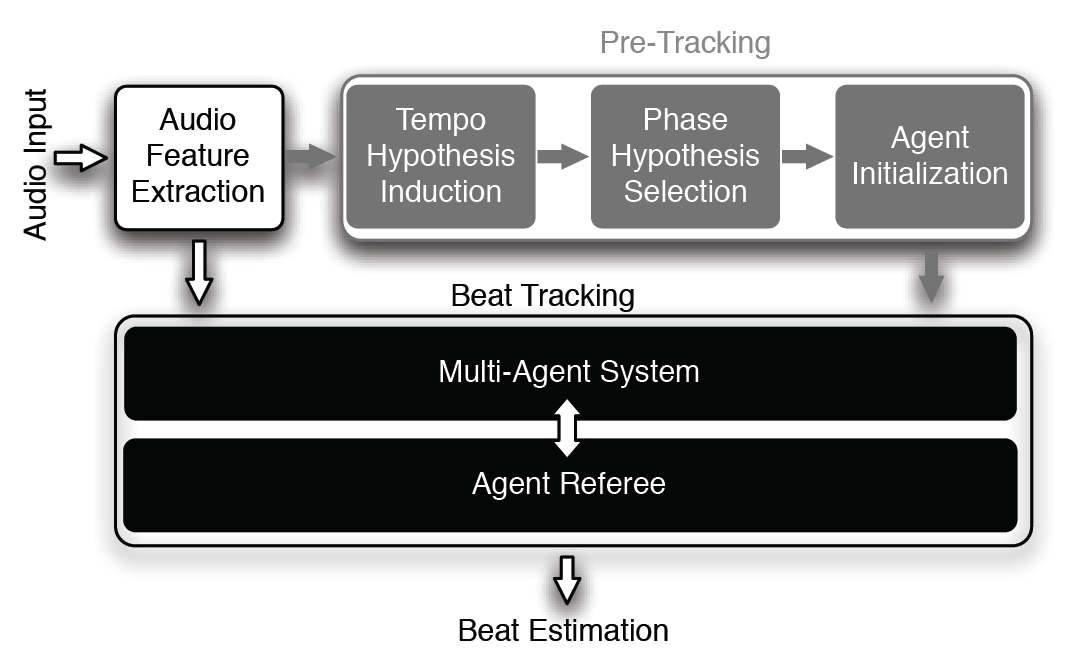
\includegraphics[width=.6\linewidth]{./pics/bloques}
\caption{Diagrama de bloques}
\label{fig:bloques}
\end{figure}

\section{Audio Feature Extraction}
En \cite{bib:feature_extraction} se evalúan distintas magnitudes para caracterizar la información más relevante para el análisis rítmico. Está fuera del alcance del presente trabajo analizar la posibilidad de evaluar distintas magnitudes, por lo que se trabajará con el \textbf{Flujo Espectral} como magnitud característica de la pieza musical.\\

El flujo espectral utiliza una representación tiempo-frecuencia de la señal basada en la trasformada corta de Fourier utilizando una ventana de Hamming, $w(m)$.\\

$X(n,k)$ representa al k-ésimo bin de frecuencia del n-ésimo frame, como se ve en la ecuación \ref{ec:x}
\begin{eqnarray}
X(n,k)=\sum\limits_{m=-\frac{N}{2}}^{\frac{N}{2}-1} x(hn+m)w(m)e^{-\frac{2\pi jmk}{N}}
\label{ec:x}
\end{eqnarray}

El flujo espectral lleva una medida del cambio en magnitud de cada \emph{bin} de frecuencia restringido a cambios positivos y sumado a lo largo de todos los \emph{bins} de frecuencia. En la ecuación \ref{ec:sf} se muestra su ecuación matemática para el cálculo.
\begin{eqnarray}
SF(n)=\sum\limits_{k=-\frac{N}{2}}^{\frac{N}{2}-1} H(|X(n,k)|-X(n-1,k)|)
\label{ec:sf}
\end{eqnarray}
donde $N=2048$ (46 $ms$ a una frecuencia de muestreo $r=44100Hz$) y el tamaño del salto es $h=441$ (10 $ms$ o 78\% de solapado). $H(x)$ es un rectificador de media onda: $H(x)=\frac{x+|x|}{2}$.


%TODO figura

\section{Pre-Tracking}
\label{sec:pretracking}

La etapa del Pre-Tracking es fundamental ya que en ella se basarán las etapas siguientes del algoritmo. Se analiza una \emph{ventana de inducción} de 5 segundos y se obtiene como salida un conjunto de agentes caracterizados por $(P_i,\phi _i, S_i) $ para cada agente $i=1\dots N$. Consta de 3 sub-etapas donde se calcula el período ($P_i$), fase ($\phi _i$) y puntaje ($S_i$) de cada agente $i$.

\subsection{Período}
La primera etapa consiste en hallar una función de periodicidad continua basada en la autocorrelación y el Flujo Espectral:
\begin{equation}
	A(\tau) = \sum\limits_{n=0}^{m}SF(n)SF(n+\tau)
	\label{ec:autocorrelacion}
\end{equation}
La segunda etapa consiste en la detección de eventos, por medio de un hallado y filtrado de picos de la función de autocorrelación descripta anteriormente (ecuación \ref{ec:autocorrelacion}). Los eventos detectados en $A(\tau)$ corresponderán con los períodos iniciales de los agentes del Pre-Tracking. El criterio propuesto para obtener dichos picos es:
\begin{equation*}
	\begin{cases}
	P_i = \arg\max_i \left\{ A(\tau) \right\}, & i=1,\dots, N\\
	A(\tau)>\delta \frac{rms(A(\tau))}{M} & 
	\end{cases}
	\label{ec:period}
\end{equation*}
$\delta$ es un umbral determinado empíricamente en $0.75$ y $M$ es un rango de tiempos definido entre [50,250] BPM.

%TODO figura y explicar que es lo q agregamos nosotros

\subsection{Fase}

Para cada $P_i$ estimado se generan $j$ hipótesis para la fase: $\phi_i^j$. Se supone fase y períodos constantes en cada ventana de análisis.\\

Se utiliza un \emph{template} de tren de pulsos isócronos para ver cuál ajusta mejor a los picos del Flujo Espectral en la ventana de inducción.\\

Utilizando un proceso de tracking simplificado como veremos en la sección \ref{sec:tracking} se selecciona el tren de pulsos que mejor ajusta los eventos detectados. Hasta este momento tenemos una pareja $(P_i,\phi _i)$ para cada agente.

\subsection{Puntaje}

A cada pareja $(P_i,\phi _i)$ se le asigna un puntaje preliminar $S_i^{raw}$ que corresponde a la suma de los errores entre los elementos del tren de pulsos y los máximos locales del Flujo Espectral, dado por la ecuación \ref{ec:ds}.\\

\begin{wrapfigure}{l}{0.45\textwidth}
	\vspace{-25pt}
	\begin{center}
	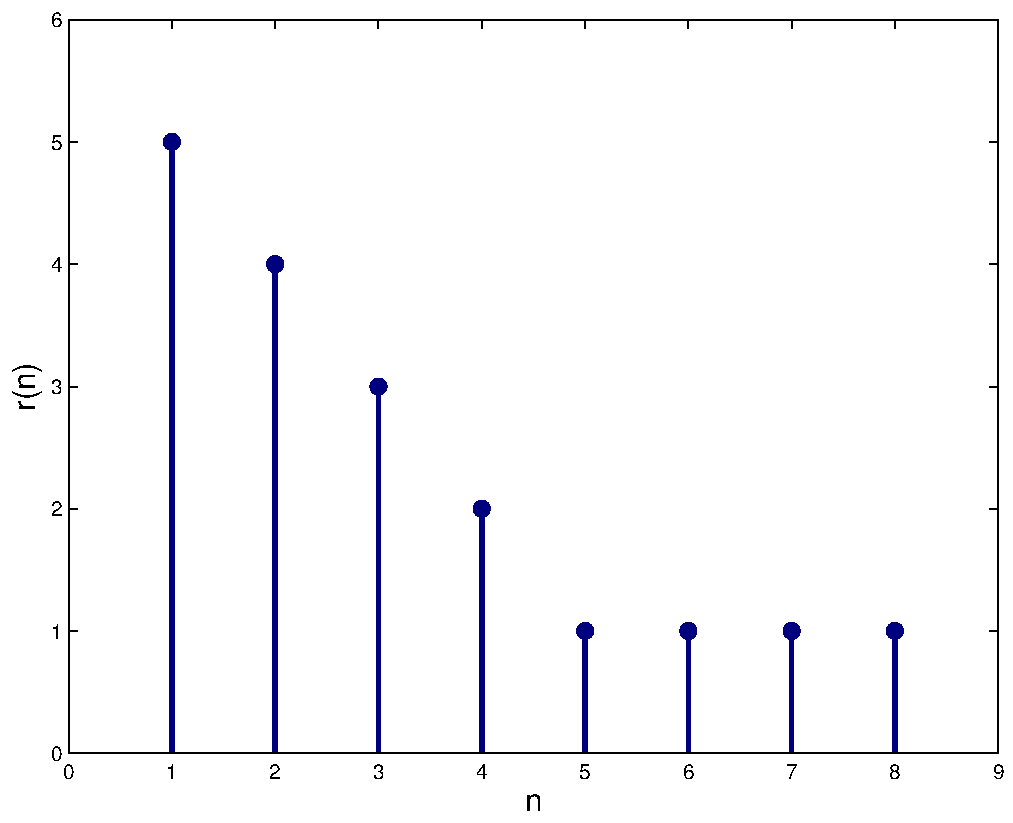
\includegraphics[width=0.4\textwidth]{./pics/r.pdf}
	\end{center}
	\vspace{-20pt}
	\caption{r(n)}
	\label{fig:r}
	\vspace{-35pt}
\end{wrapfigure}

Luego considerando relaciones métricas entre pares de hipótesis de período ($n_{ij}$), se actualiza el puntaje a:
$$S^{rel}_i=10S_i^{raw}+\mathop{\sum\limits_{j=0}^{N}}_{j \neq i}r(n_{ij})S_j^{raw}$$ donde 
$$r(n)= \begin{cases}
6-n, & 1\leq n \leq 4\\
1, & 5\leq n \leq 8\\
0, & en\;otro\;caso
\end{cases}
$$

que también se puede ver representada en la figura \ref{fig:r}. El resultado de aplicar la función $r(n)$ es favorecer todos los agentes que tengan múltiplos enteros uno de otro.\\

Por último el puntaje final está dado por:
\begin{equation}
S_i=\frac{S_i^{rel}}{\max S_i^{rel}}\max S_i^{raw}
\label{ec:S}
\end{equation}

Tenemos entonces un conjunto de agentes, donde cada uno de ellos está caracterizado por una tríada $(P_i,\phi _i,S_i)$ que serán utilizados como hipótesis iniciales para la etapa de \textbf{Tracking}.

\section{Beat-Tracking}
\label{sec:tracking}

La idea de la etapa de Tracking es supervisar flujo de entrada de los picos detectados del Flujo Espectral y mantener un buen balance entre inercia y rapidez de la respuesta ante cambios.\\

Cada predicción es evaluada respecto de su desviación al máximo local correspondiente en los datos observados, considerando una ventana como se la mostrada en la figura \ref{fig:grafica}, donde se consideran 2 intervalos de tolerancia:
\begin{itemize}
\item \emph{inner}: $T_{in}\in[T_{in}^l,T_{in}^r]$ con $T_{in}^l=T_{in}^r=46.4ms$ para manejar pequeñas desviaciones de fase y período
\item \emph{outer}: $T_{out}\in[T_{out}^l,T_{in}^l] \bigcup [T_{in}^r,T_{out}^r]$ con $T_{out}^l=0.2\;P_i$ y $T_{out}^r=0.4\;P_i$ para contemplar eventuales cambios repentinos de tiempo. La asimetría refleja una mayor tendencia a disminuir el tempo.\\
\end{itemize}

\begin{figure}[h!]
  \begin{center}
  \vspace*{-10pt}
  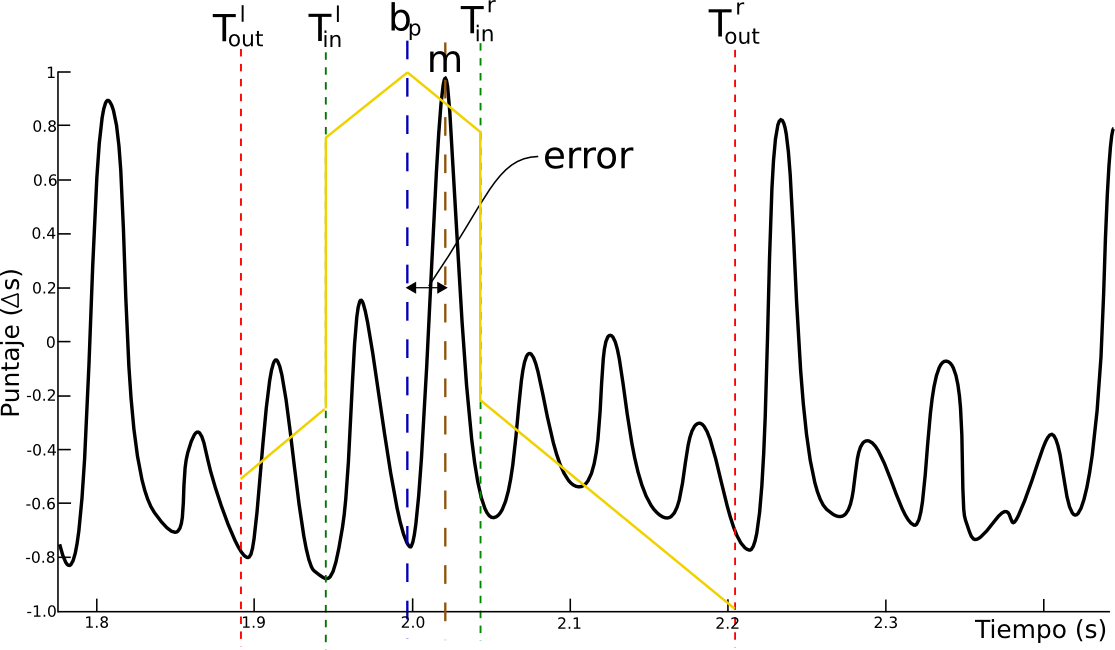
\includegraphics[width=.8\textwidth]{./pics/graficamejor.png}
  \end{center}
  \vspace{-10pt}
  \caption{Niveles de tolerancia}
  \label{fig:grafica}
\end{figure}

En consecuencia aparecen 2 claros escenarios distintos: o bien que el máximo local del Flujo Espectral se encuentre en la región \emph{inner}, o bien que se encuentre en la región \emph{outer}.\\

\begin{itemize} \item Máximo local en región \emph{inner}\end{itemize}
En este caso se considera que el agente está siguiendo los beats de la pieza de buena manera y lo único que se realiza es un ajuste fino de período y fase según sigue:
$$
\begin{cases}
P_i = P_i+0.25\;error\\
\phi_i = \phi_i+0.25\;error
\end{cases}
$$

\begin{itemize} \item Máximo local en región \emph{outer} \end{itemize}
Este caso corresponde a desviaciones mayores que el caso anterior, donde el agente mantiene su período y fase pero para hacer frente a variaciones de tempo repentinas crea 3 ``hijos'' ($C_1$,$C_2$,$C_3$) para seguir 3 alternativas posibles combinando variaciones de \emph{timing} (fase) y \emph{tempo} (período), según sigue:\\
\footnotesize
$$
C_1:
\begin{cases}
P_{C_1}=P_i\\
\phi _{C_1}=\phi _i + error + P_{C_1}
\end{cases}
, \exists m \in T_{out}
$$
$$
C_2:
\begin{cases}
P_{C_2}=P_i+error\\
\phi _{C_2}=\phi _i + error + P_{C_2}
\end{cases}
, \exists m \in T_{out}
$$
$$
C_3:
\begin{cases}
P_{C_3}=P_i+0.5\;error\\
\phi _{C_3}=\phi _i +0.5\;error + P_{C_3}
\end{cases}
, \exists m \in T_{out}
$$

\normalsize

Para que los hijos tengan competitividad respecto al resto de los agentes, se los inicializa con un puntaje igual al 90\% del puntaje del ``padre'' en ese instante.

\subsection{Matado de agentes}

En cualquier punto del análisis, algunas situaciones dan por finalizada la operación de un agente, con los criterios que se explican a continuación:

\begin{itemize}
\item \emph{Replacement}: un agente es matado si llegado al límite de agentes (fijado en 30), es el peor de todos y su puntaje es menor al de otro agente creado más recientemente.
\item \emph{Redundancy}: para mejorar la eficiencia del algoritmo un agente es matado si está duplicando el trabajo de otro con mayor puntaje. Por duplicación de trabajo se entiende que la diferencia entre los períodos no debe ser mayor a $11.6\;ms$ y la diferencia entre las fases no debe superar los $23.2\;ms$.
\item \emph{Obsolence}: un agente es matado si la diferencia entre su puntaje con el mejor agente es mayor al 80\% del mejor puntaje
\item \emph{Loss}: un agente es matado si parece estar ``perdido'', sugerido una cantidad (fijada en 8) de veces consecutivas que la predicción del beat esté por afuera de la región \emph{inner}.
\end{itemize}

\subsection{Agent Referee}

En la versión causal el \emph{referee} va determinando en cada instante cuál es el mejor agente. Mantiene una continua evaluación y le va asignando un puntaje a cada agente respecto a qué tan bueno es el matcheo entre los datos que van llegando y la prediccion del beat. La variación de puntaje en cada instante está dada por la ecuación \ref{ec:ds}.\\

\begin{equation}
\begin{cases}
\Delta s = \left(1-\frac{|error|}{T^r_{out}} \right)\frac{P_i}{P_{max}}SF(m), & \exists m \in T_{in}\\
\Delta s = -\left(\frac{|error|}{T^r_{out}} \right)\frac{P_i}{P_{max}}SF(m), & \exists m \in T_{out}
\end{cases}
\label{ec:ds}\\
\end{equation}
\\
$b_p$ es la predicción del beat, $m$ el máximo correspondiente del Flujo Espectral, y $P_{max}$ el período máximo permitido (correspondiente a $250\;BPM$). El cociente $P_i/P_{max}$ es utilizado para normalizar la función puntaje por el período $P_i$ y es utilizado como una manera de disminuir el puntaje de los agentes más rápidos, que de otra manera tendería a aumentar dado que tienen una mayor cantidad de predicciones de beat. La utilización de un puntaje negativo cuando la predicción cae fuera de la región \emph{inner} infiere una penalización al agente correspondiente.\\

\chapter{Resultados}

\section{Detalles de implementación}
\label{sec:nosotros}

En esta sección se presentan algunos detalles en los cuales fue necesario ahondar el estudio para la correcta implementación del algoritmo presentado en la sección \ref{sec:metodologia}, y que resultan interesante destacarlos y documentarlos.\\

A la hora de realizar el tracking es necesario computar el error entre la predicción del beat y el máximo del Flujo Espectral, lo cual puede hacerse de diferentes maneras y no se brinda información acerca de cómo está implementado en \cite{bib:el_posta}. Se plantean 2 casos posibles:
\begin{enumerate}
\item Recorrer los máximos del flujo espectral e ir comparando con la predicción del beat para cada agente y hallar el error
\item Recorrer las predicciones de beat para cada agente e ir comparando con el máximo del Flujo Espectral correspondiente
\end{enumerate}
Para la implementación se decidió utilizar la primera opción. Se recorre entonces para cada pico del flujo espectral cada uno de los agentes considerando su predicción de beat.

\begin{wrapfigure}{l}{0.55\textwidth}
	\vspace{-25pt}
	\begin{center}
	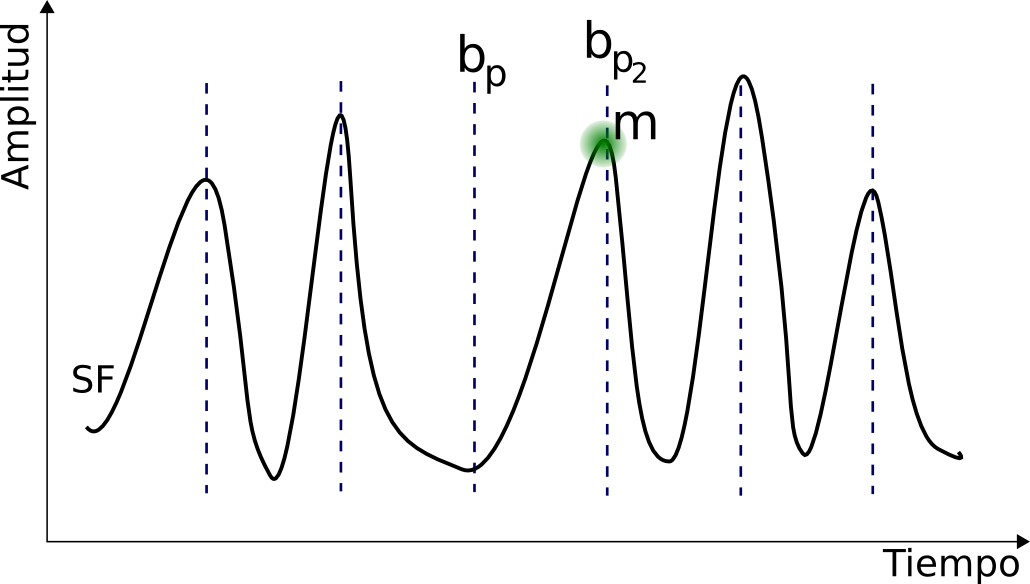
\includegraphics[width=0.5\textwidth]{./pics/caso1.png}
	\end{center}
	\vspace{-20pt}
	\caption{Caso 1}
	\label{fig:caso1}
\end{wrapfigure}

Una de las primeras dificultades que se encontraron fue que cuando faltaban algunos picos en el Flujo Espectral los agentes morían rápidamente debido a que la predicción cae muy lejos del evento. Dicha situación se representa en la figura \ref{fig:caso1}. Las líneas punteadas representan las predicciones de un agente ejemplo. A la vista está que el agente aproxima de buena manera a todos de los picos del Flujo Espectral, pero parece faltar un pico en las cercanías de $b_p$. Al comparar el pico $m$ con la predicción $b_p$, el error es tan grande que causa la terminación del agente. Para evitar esta terminación lo que se hace es comparar $m$ con $b_{p_2}=b_p+P$ en lugar de con $b_p$.

\begin{wrapfigure}{r}{0.55\textwidth}
	\vspace{-25pt}
	\begin{center}
	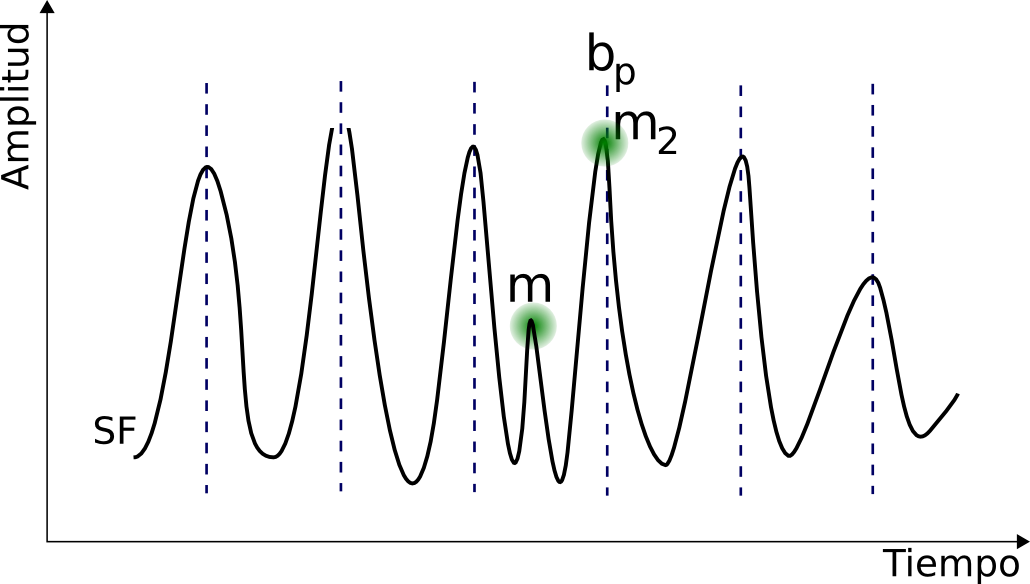
\includegraphics[width=0.5\textwidth]{./pics/caso2.png}
	\end{center}
	\vspace{-20pt}
	\caption{Caso 2}
	\label{fig:caso2}
\end{wrapfigure}

Una segunda dificultad, muy estrechamente vinculada con la anterior consiste en la aparición de máximos intermedios \emph{espúreos} que también causan la muerte de un buen agente. La situación se representa en la figura \ref{fig:caso2}. Al comparar el máximo $m$ con la predicción de beat $b_p$ se obtiene un error demasiado grande que causa la muerte del agente. Para solucionar esta situación lo que se hace es comparar el error entre $b_p$ y $m_2$ (el siguiente máximo del Flujo Espectral) y si este error es menor al primero, no se efectúa ninguna acción sobre ese agente. De todas formas es interesante destacar que al continuar el algoritmo, cuando sea el turno del máximo $m_2$ se realizará el proceso de tracking normalmente.\\

El trabajo en el que nos basamos está pensado para correr en tiempo real, pero como la propuesta nuestra no lo requería nos tomamos algunas libertades que enlentecen el algoritmo. La más importante es \emph{no matar a los agentes que caen fuera de la región ``outer''}. De hecho lo que se implementó es matarlos si caen fuera de dicha región consecutivamente más de una cantidad fija de veces.\\

Para elegir el agente ganador tomamos la idea de que utiliza \emph{Dixon} en el \emph{BeatRoot} (\cite{bib:dixon}), donde se utiliza un referee que decide al final del proceso de tracking. Se basa en la idea que al ir teniendo buenos puntajes a lo largo del tracking, el agente que tenga mayor puntaje al finalizarlo será el mejor agente global.

\section{Señales sintéticas}

Como primer prueba para testear el algoritmo implementado se generan diversas señales sintéticas con período constante. Para ello se convolucionan el sonido de un platillo de batería con un tren de pulsos de frecuencia constante. La prueba siguiente, también sintética consiste en generar una señal con frecuencia variando linealmente a lo largo del tiempo para analizar la performance del algoritmo en el tracking del período variante de una señal.\\

Como primer ejemplo se presenta el caso de una señal de período constante en $90\;BMP$. Los resultados se muestran en las figuras \ref{fig:90BPM}.

\begin{figure} [h!]
\centering
  \subfloat[Autocorrelación del Flujo Espectral]{\label{fig:bpm90autocorr} \centering
  		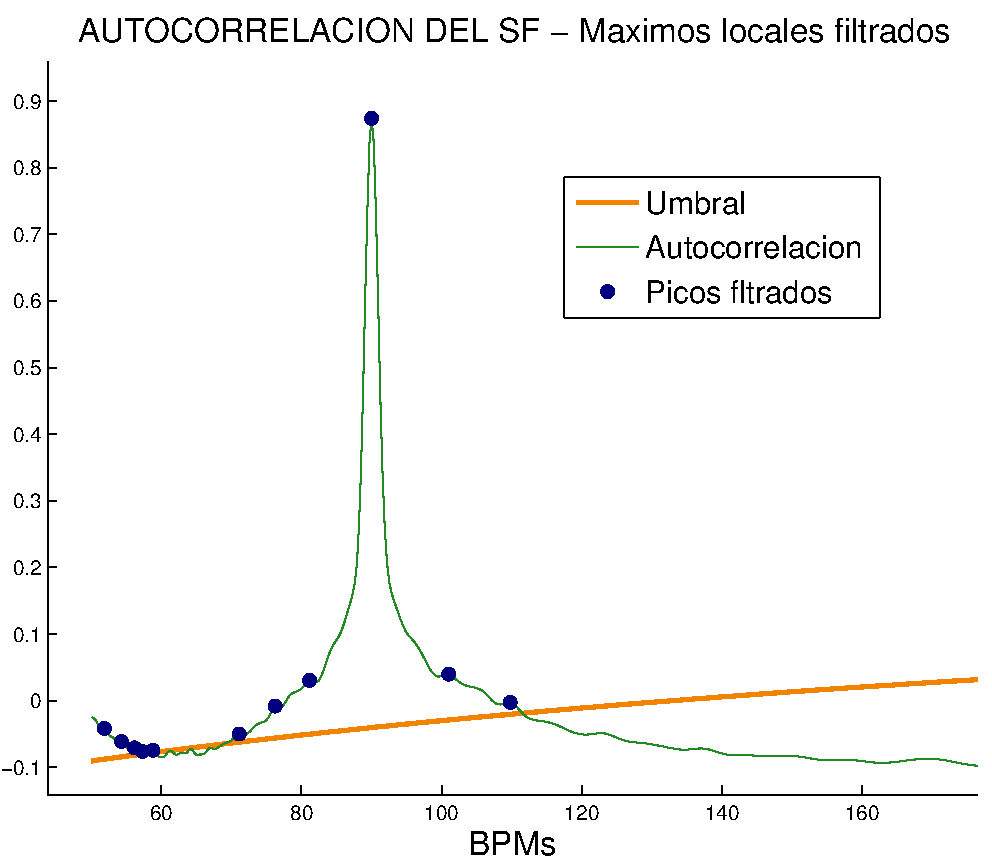
\includegraphics[width=.5\textwidth]{./pics/bpm90autocorr.pdf}} 
  \subfloat[Beats detectados sobre la señal]{\label{fig:bpm90beats} 
  		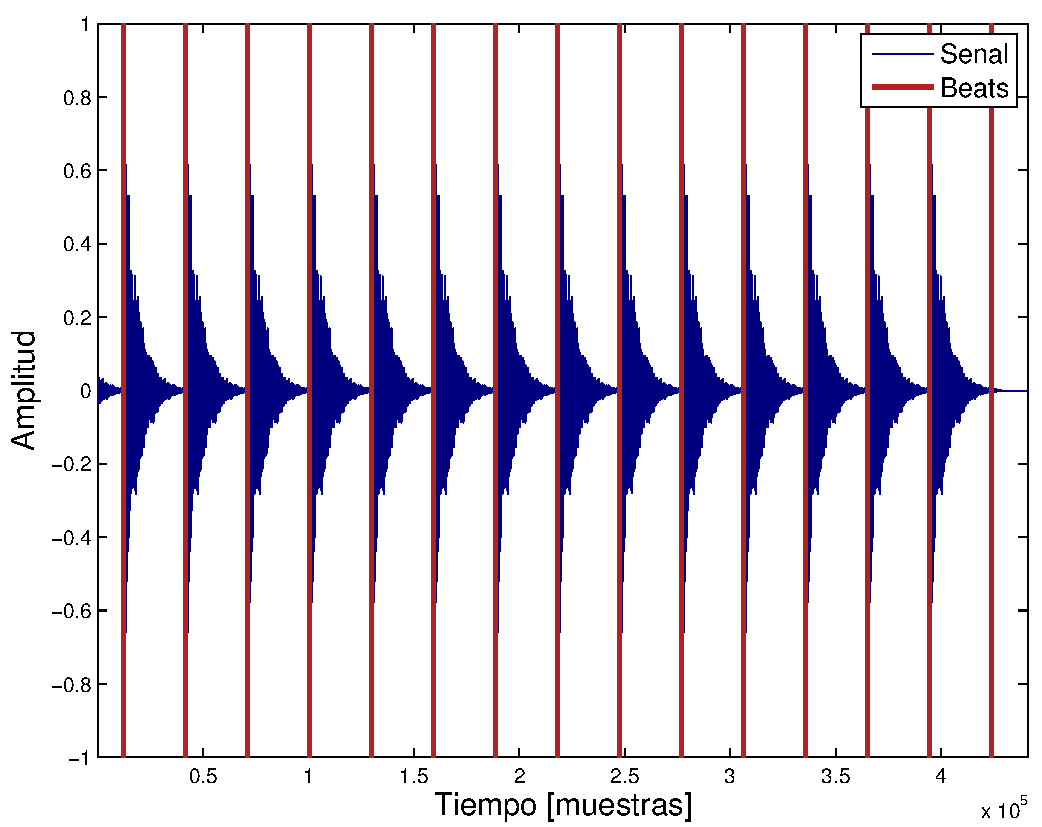
\includegraphics[width=.5\textwidth]{./pics/bpm90beats.pdf}}
  \caption{Señal sintética de 90 BPM}
  \label{fig:90BPM}
\end{figure}

La figura \ref{fig:bpm90autocorr} muestra la autocorrelación del flujo espectral calculado en la \emph{ventana de inducción} mencionada en la sección \ref{sec:pretracking} del Pre-Tracking. Se puede apreciar claramente que el pico marcado que aparece en la figura corresponde con un período de 90BPM, coincidiendo perfectamente con el período de la señal sintética generada. Se puede decir entonces que el Pre-Tracking captó perfectamente el período del beat. Se muestra también el umbral utilizado para filtrar los máximos locales del Flujo Espectral detectados. Por otro lado en la figura \ref{fig:bpm90beats} se muestra una representación de la señal de audio, y sobrepuesta a ella una línea roja en la posición de cada beat detectado. Se puede corroborar el perfecto funcionamiento del algoritmo en este caso.\\

Para analizar la capacidad de adaptación del algoritmo a una pieza musical con tempo variante se genera una señal sintética con período variante entre 90BPM y 100BPM. Los resultados se muestran en la figura \ref{fig:tempovariante}.

\begin{figure} [h!]
\centering
  \subfloat[Beats detectados sobre la señal]{\label{fig:bpm90a100beats} \centering
  		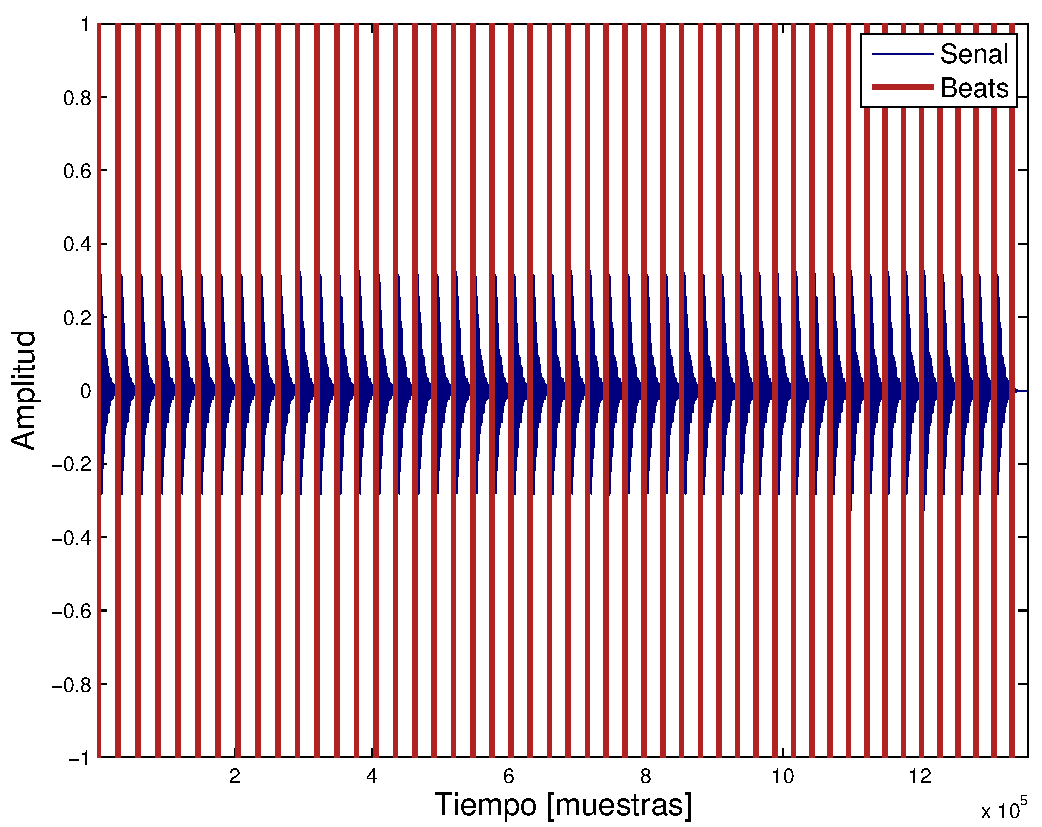
\includegraphics[width=.5\textwidth]{./pics/bpm90a100beats.pdf}} 
  \subfloat[Evolución del tempo]{\label{fig:bpmvariable} 
  		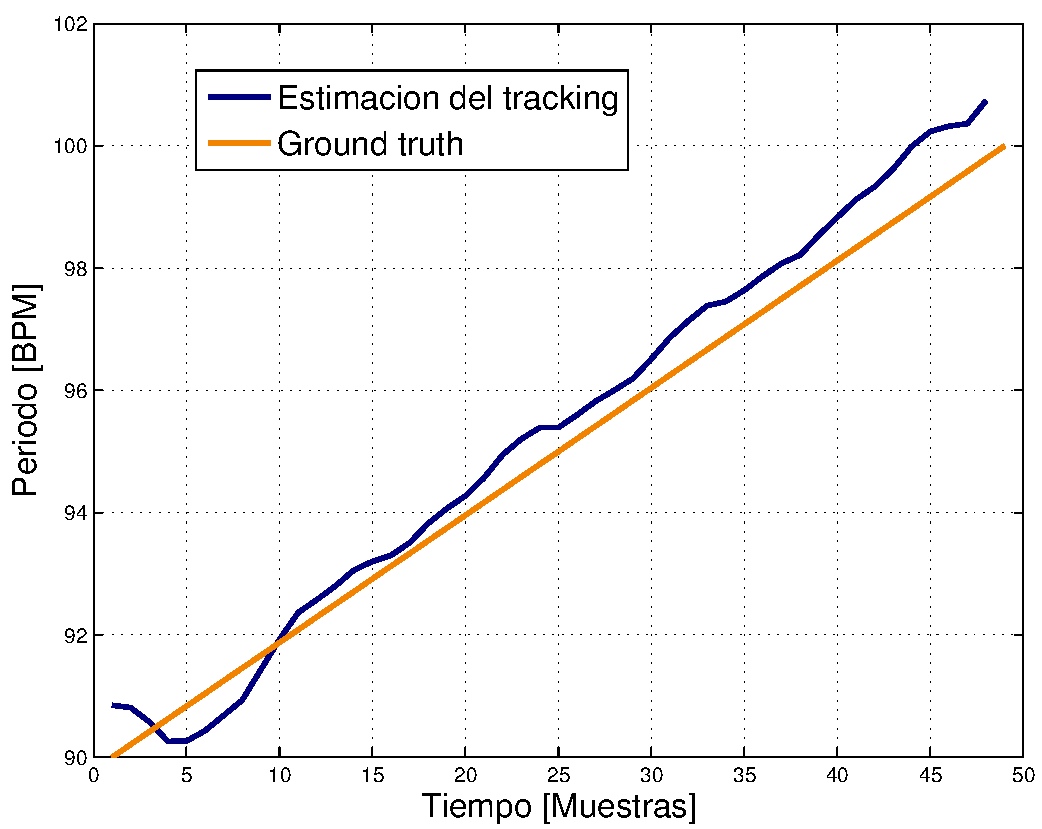
\includegraphics[width=.5\textwidth]{./pics/bpmvariable.pdf}}
  \caption{Señal sintética con tempo variante en forma lineal}
  \label{fig:tempovariante}.
\end{figure}

En la figura \ref{fig:bpm90a100beats} se muestra la señal sintética original con los beats sobrepuestos, donde se puede observar a grandes rasgos que se realiza el tracking en forma exitosa. Por otro lado en la figura \ref{fig:bpmvariable} se puede observar con más detalle la evolución del tempo a lo largo del tiempo. Comparando ambas curvas se puede afirmar que, a menos de un error de alrededor de $0.5\;BPM$, se realiza un tracking exitoso del tempo de la pieza.\\

Una vez realizadas las pruebas sintéticas y corroborado el funcionamiento en situaciones controladas, se procede a testear el algoritmo implementado en situaciones reales, como se pasa a describir en la siguiente sección.

\section{Señales reales}

Si bien el pasaje de casos sintéticos a reales siempre conlleva el agregado de una cantidad de no idealidades de la señal que pueden causar situaciones no previstas y así un mal desempeño del algoritmo, en este caso la performance alcanzada continúa siendo considerablemente buena. De todas formas se presentan casos donde el algoritmo funciona de forma correcta y donde tiene alguna dificultad.

\subsection{Caso de buen funcionamiento}

En esta sección se presentan los resultados para una pieza musical donde el comportamiento del algoritmo coincide completamente con el \emph{ground truth} de la señal.\\

\begin{wrapfigure}{l}{0.55\textwidth}
	\vspace{-25pt}
	\begin{center}
	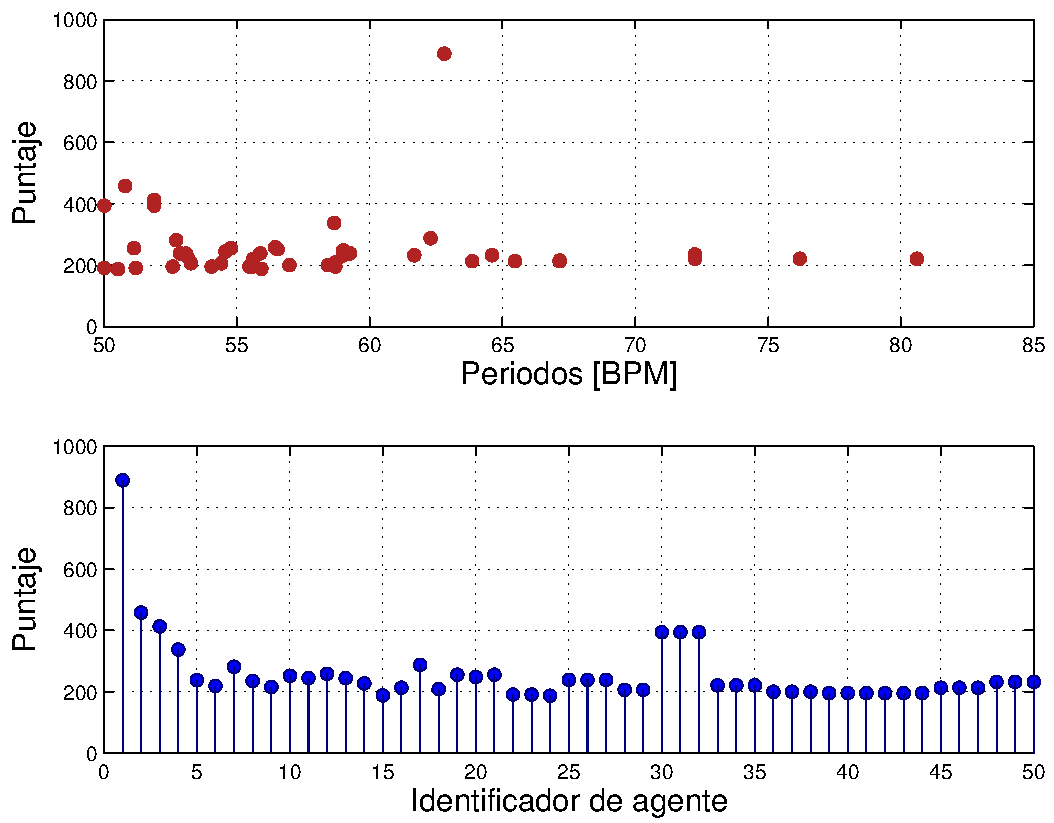
\includegraphics[width=0.5\textwidth]{./pics/datos_2_2_A_agents.pdf}
	\end{center}
	\vspace{-20pt}
	\caption{Agentes finales}
	\label{fig:datos_2_2_A_agents}
\end{wrapfigure}

En la figura \ref{fig:datos_2_2_A_agents} se muestra la configuración de los agentes al terminar el tracking sobre toda la pieza musical. Cada punto en la gráfica representa un agente. En la gráfica de arriba se muestra el puntaje final de cada agente en función de su período final, mientras que en la gráfica de abajo se muestra lo mismo pero en función del identificador de cada agente. El número de agente da una idea de la ``edad'' de cada agente. Se puede observar en dicha figura que el $1^{er}$ agente tiene un puntaje ligeramente superior que el resto, por lo que será agente ganador para esta pieza.\\

En la figura \ref{fig:datos_2_2_A} se muestran más resultados obtenidos para la pieza musical en cuestión. En la figura \ref{fig:datos_2_2_A_autocorr} se muestra la autocorrelación del Flujo Espectral en la \emph{ventana de inducción} en función del período en BPM y en la figura \ref{fig:datos_2_2_A_beats_bien} se muestra la señal original con los beats detectados sobrepuestos.\\

\begin{figure} [h!]
\centering
  \subfloat[Autocorrelación del Flujo Espectral y filtrado de picos]{\label{fig:datos_2_2_A_autocorr} \centering
  		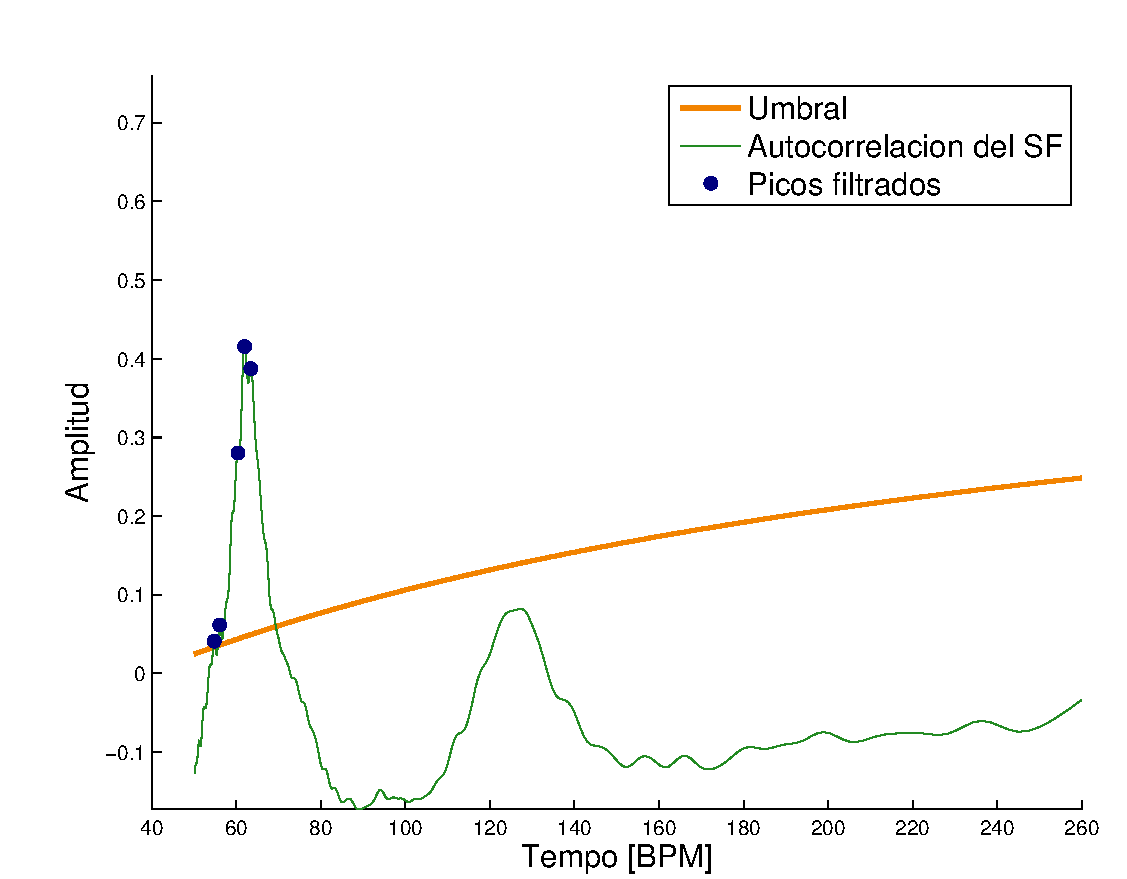
\includegraphics[width=.47\textwidth]{./pics/datos_2_2_A_autocorr.pdf}} 
  \subfloat[Beats detectados sobre la señal de audio original]{\label{fig:datos_2_2_A_beats_bien} 
  		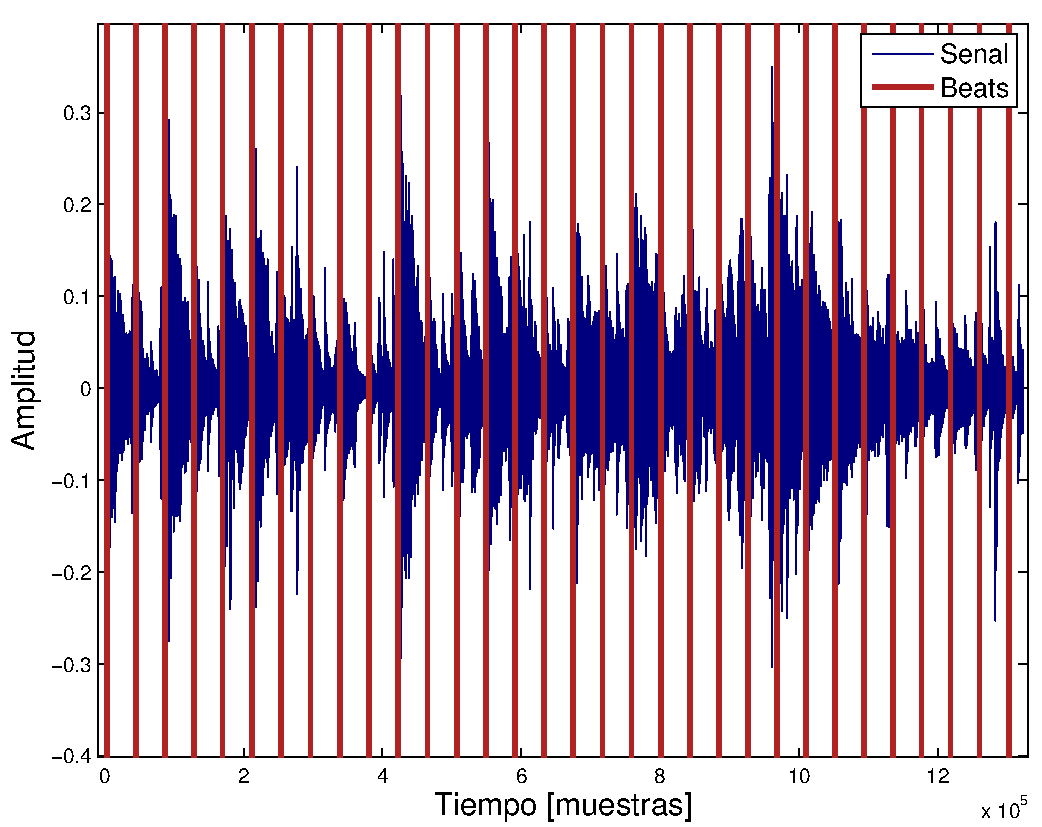
\includegraphics[width=.47\textwidth]{./pics/datos_2_2_A_beats_bien.pdf}}
  \caption{}
  \label{fig:datos_2_2_A}
\end{figure}

Si se observa el período del agente ganador mostrado en la figura \ref{fig:datos_2_2_A_agents} y se lo compara con el \emph{tempo} del mayor pico de la autocorrelación mostrado en la figura \ref{fig:datos_2_2_A_autocorr} se advierte una gran similitud, lo cual sugiere que el agente ganador viene de una familia inicializada por un agente creado en el pre-tracking correspondiente a dicho pico. En este caso el pre-tracking logró estimar de muy buena manera el tempo de la pieza musical y el agente se mantuvo durante toda la pieza ajustando levemente su \emph{tempo} y \emph{timing} y acumulando un buen puntaje.\\

Por otra parte se puede corroborar visualmente observando la figura \ref{fig:datos_2_2_A_beats_bien} que en cada ataque de la pieza musical se presenta un beat detectado, lo cual corrobora el buen funcionamiento del algoritmo.\\

Se realizaron además algunas pruebas cuantitativas utilizando las medidas \emph{Continuity based} y \emph{F-Measure} obteniendo el siguiente resultado:

\begin{verbatim}
---------------------------------------------------------------------
Performance:
        	Cont-Based:	 cC:	100.00	cT:	100.00	aC:	100.00	aT:	100.00
        	F-Mesure:     f:	 94.44	 p:	94.44   r:	94.44 	 a:	89.47
---------------------------------------------------------------------
\end{verbatim}

Por último y no menos importante es interesante destacar el resultado auditivo de la señal de salida, el cual parece comportarse de manera perfecta a lo largo de la pieza musical.


\subsection{Caso de funcionamiento comprometido}
\label{sec:andamal}

En esta sección se presenta un caso en el que el desempeño del algoritmo tiene algunas dificultades, aunque en líneas generales la performance resulta aceptable.\\

\begin{wrapfigure}{l}{0.55\textwidth}
	\vspace{-25pt}
	\begin{center}
	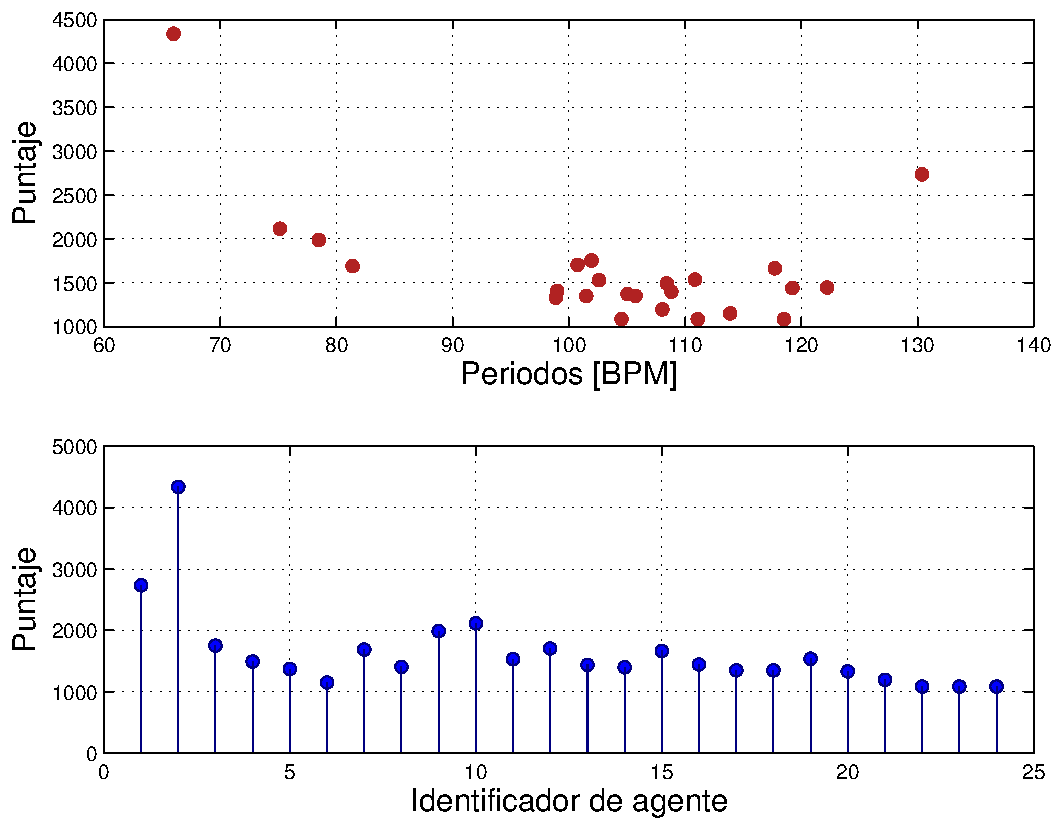
\includegraphics[width=0.5\textwidth]{./pics/datos_2_14_A_agents.pdf}
	\end{center}
	\vspace{-20pt}
	\caption{Agentes finales}
	\label{fig:datos_2_14_A_agents}
	\vspace{-35pt}
\end{wrapfigure}

En la figura \ref{fig:datos_2_14_A_agents} se muestra la configuración de los agentes al finalizar el tracking sobre toda la pieza musical. Se advierte fácilmente que hay 2 agentes que tienen un puntaje ligeramente superior al del resto y que sus tempos son uno aproximadamente el doble del otro: el agente 1 con tempo 130 BPM y el agente 2 con tempo 65 BPM.\\

He aquí un problema típico mucho más general que su aplicación a este caso de estudio. Es un problema ocasionado al tratar de computar automáticamente en una computadora algunas características que son intrínsecamente semánticas y por tanto humanas. Incluso el seguimiento del beat puede variar dependiendo de la persona, mientras que algunos pueden marcar un determinado tempo, otros pueden marcar el doble o la mitad. En este caso el consenso tomado del \emph{ground truth} dice que el agente que mejor captura el tempo de la pieza musical es el agente número 1. Como salida del algoritmo implementado el mejor agente resulta ser el agente número 2.\\

\begin{figure} [h!]
\centering
  \subfloat[En función de las muestras]{\label{fig:datos_2_14_A_autocorr} \centering
  		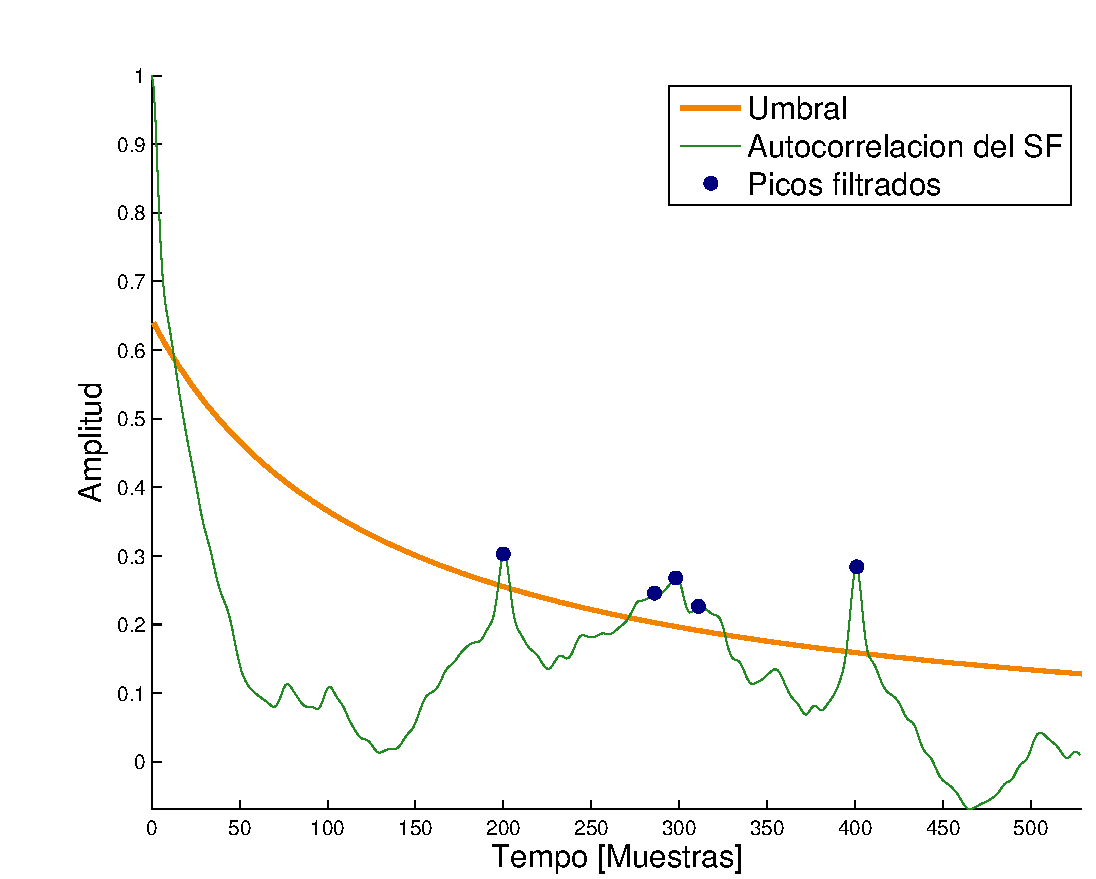
\includegraphics[width=.5\textwidth]{./pics/datos_2_14_A_autocorr.pdf}} 
  \subfloat[En función del período en BPM]{\label{fig:datos_2_14_A_autocorr2} 
  		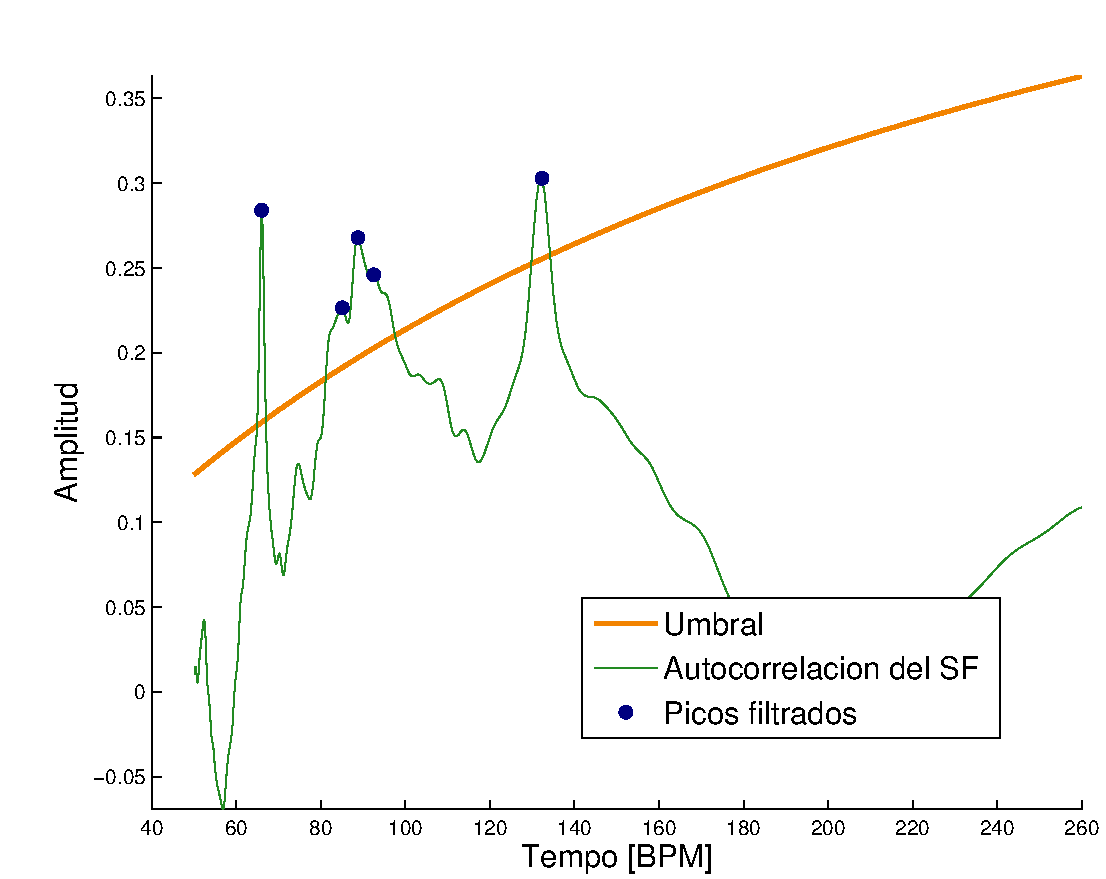
\includegraphics[width=.5\textwidth]{./pics/datos_2_14_A_autocorr2.pdf}}
  \caption{Autocorrelación del Flujo Espectral}
  \label{fig:datos_2_14_A_autocorrelaciones}
\end{figure}

En la figura \ref{fig:datos_2_14_A_autocorrelaciones} se muestra la autocorrelación del Flujo Espectral en la ventana de inducción del pre-tracking. Se puede observar que tanto el agente 1 como el 2 son inicializados en esta etapa ya que se advierten 2 claros picos, uno cerca de 65 BPM y otro cerca de 130 BPM.\\

Por último en la figura \ref{fig:datos_2_14_A_beats} se muestran los resultados obtenidos si se elige como mejor agente al número 2 (figura \ref{fig:datos_2_14_A_beats_lento}), y si se elige al número 1 (figura \ref{fig:datos_2_14_A_beats_bien}).\\

\begin{figure} [h!]
\centering
  \subfloat[Agente número 2]{\label{fig:datos_2_14_A_beats_lento} \centering
  		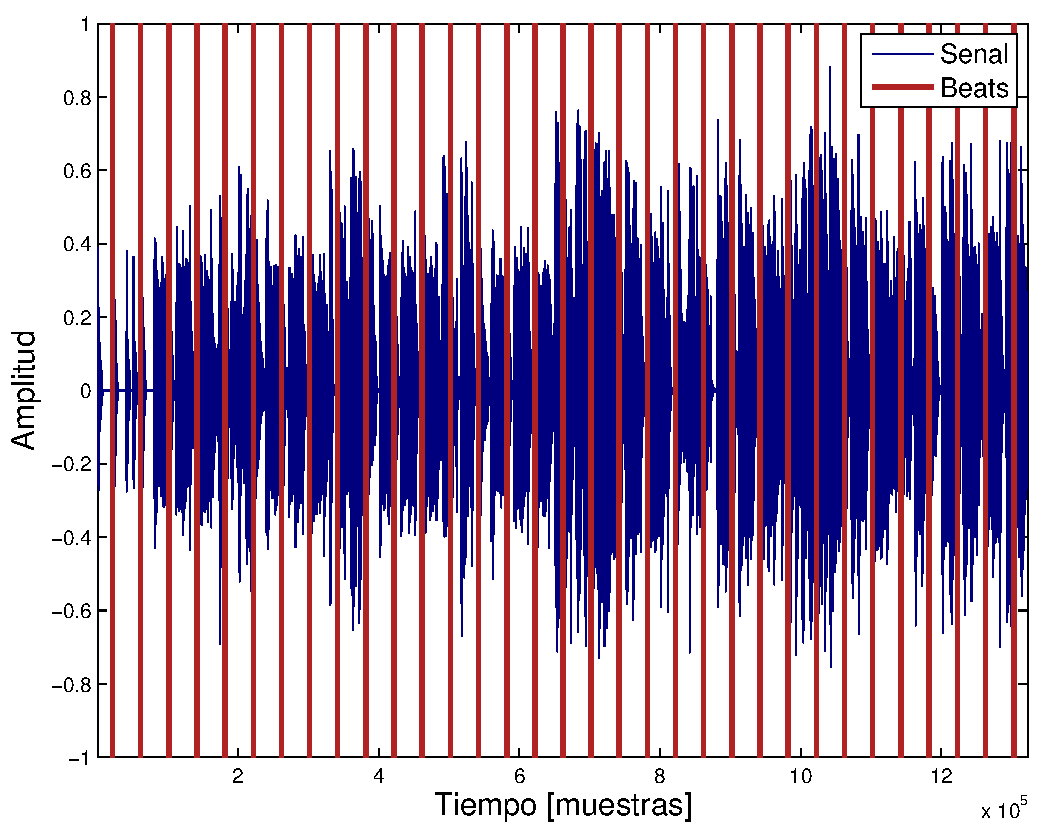
\includegraphics[width=.5\textwidth]{./pics/datos_2_14_A_beats_lento.pdf}} 
  \subfloat[Agente número 20]{\label{fig:datos_2_14_A_beats_bien} 
  		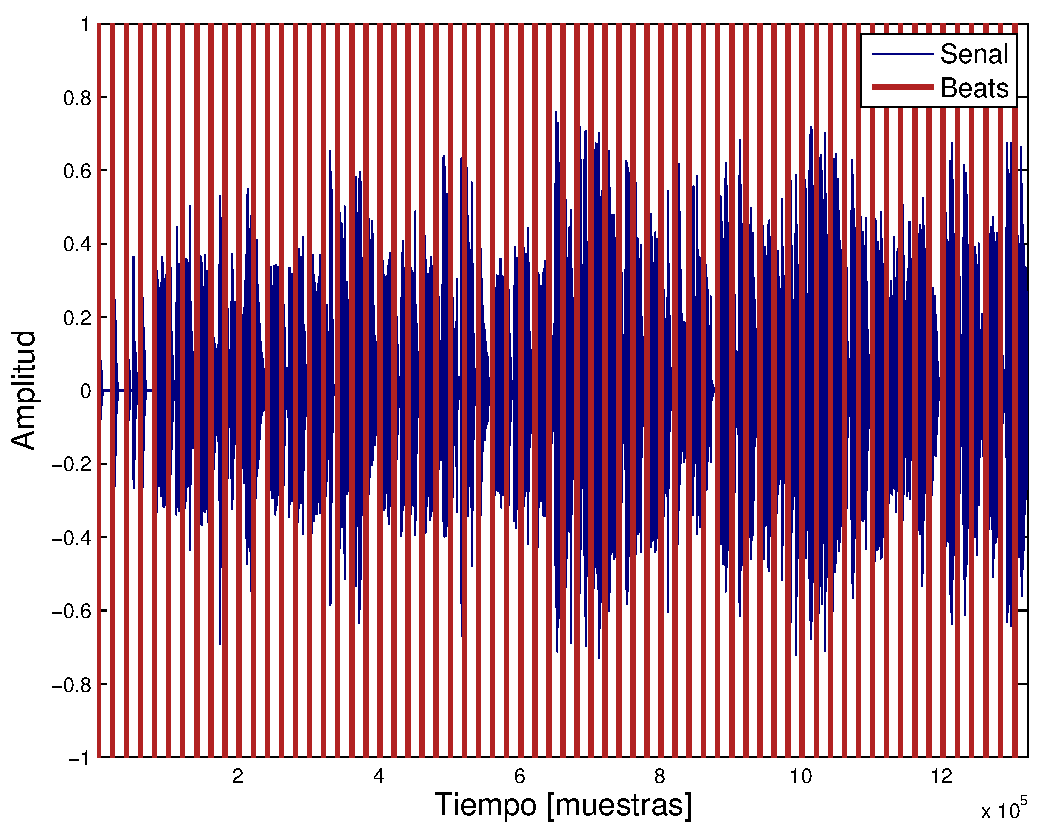
\includegraphics[width=.5\textwidth]{./pics/datos_2_14_A_beats_bien.pdf}}
  \caption{Beats detectados}
  \label{fig:datos_2_14_A_beats}
\end{figure}

En este caso es muy difícil darse cuenta visualmente observando las imágenes de la figura \ref{fig:datos_2_14_A_beats} cuál de los dos sigue de mejor forma al beat, pero si analizamos auditivamente los resultados habrá consenso entre la mayoría de las personas que el agente número 20 sigue de mejor forma el beat de esta pieza musical.\\

Si se elije como mejor agente al número 2 la performance alcanzada será:
\begin{verbatim}
---------------------------------------------------------------------
Performance agente 2:
        	Cont-Based:	 cC:	00.00	cT:	00.00	 aC:	100.00	aT:	100.00
        	F-Mesure: 	   f:	67.47  p:	100.00	 r:	50.91	  a:	50.91
---------------------------------------------------------------------
\end{verbatim}
Se puede ver que algunas medidas de desempeño penalizan fuertemente este tipo de errores mientras que otras los admiten de distintas formas y lo penalizan en mayor o menor medida.\\

Por último si se elije como mejor agente al número 1 la performance alcanzada será perfecta:
\begin{verbatim}
---------------------------------------------------------------------
Performance agente 1:
        	Cont-Based:	 cC:	100.00	cT:	100.00	aC:	100.00	aT:	100.00
        	F-Mesure:	    f:	100.00	 p:	100.00	 r:	100.00	 a:	100.00
---------------------------------------------------------------------
\end{verbatim}

En este caso la performance del algoritmo hubiera sido perfecta.


\section{Conclusiones}

Como primer punto se debe destacar que una gran cantidad de detalles de implementación no están documentados en el \emph{paper} que se basó el presente trabajo (\cite{bib:el_posta}), lo cual ocasionó una serie de dudas y  por tanto la toma de las decisiones que nos parecieron más adecuadas, mencionadas en la sección \ref{sec:nosotros}.\\

Como conclusión general se puede decir que se obtuvieron buenos resultados, en algunas piezas musicales los resultados son excelentes, y en otras ``más difíciles'' no tanto, pero en general parecen ser aceptables. El trabajo \cite{bib:el_posta} consta además de un software disponible en \emph{Marsyas framework} bajo licencia GPL. Comparando los resultados de esta implementación con los resultados del presente trabajo debemos decir que obtuvimos un desempeño algo inferior.\\

El algoritmo además de arrojar buenos resultados en la mayoría de los casos, está programado con buena robustez ante diferentes características de las señales de entrada, poniendo siempre umbrales variables y dependientes de características propias de la señal y teniendo algunos cuidados especiales retroalimentando información obtenida de la señal misma para cambiar dinámicamente algunos valores.\\

Como se mostró en la sección \ref{sec:andamal}, se cometen algunos errores a la hora de elegir el agente ganador. En esta materia se puede pensar en alguna técnica para agregar que permita, cambiando el criterio de elección del agente ganador, obtener resultados más fieles a la realidad.\\

Es interesante destacar que se logró un buen equilibrio entre la inercia a los cambios transitorios que puedan existir en una pieza musical y la rapidez de adaptación a cambios de tempo. Por ejemplo en pasajes donde se producen silencios o cortes abruptos pasajeros en una pieza musical, el algoritmo sigue marcando el beat constantemente, como es de esperar.\\

En definitiva se puede decir que la idea de varios agentes compitiendo por seguir el tempo de la canción lo mejor posibles es una buena técnica que arroja buenos resultados. La manera de puntuar a los agentes parece estar muy bien lograda, ya que favorece a los mejores agentes. De todas formas pueden surgir algunas complicaciones a la hora de elegir cuál es el ganador, pero en general se logra dar en buena forma el salto semántico desde el automatismo a la percepción auditiva rítmica del ser humano.

\begin{thebibliography}{99}
\begin{small}

\bibitem{bib:el_posta}Jo\~ao Lobato Oliveira, Fabien Gouyon, Luis Gustavo Martins, Luis Paulo Reis, IBT: A real time tempo and beat tracking system, In \emph{11th International Society for Music Information Retrieval Conference, ISMIR}, 2010.

\bibitem{bib:dixon}S. Dixon. Automatic extraction of tempo and beat from
expressive performances. In \emph{Journal of New Music Research, 30(1):39–58}, 2001.

\bibitem{bib:feature_extraction}S. Dixon. Onset detection revisited. In \emph{in Proceedings of the 9th International Conference on Digital Audio Effects}, pages 133–13, Montreal, Canada, 2006.

\bibitem{bib:y_asi}F. Gouyon, P. Herrera, and P. Cano. Pulse-dependent analyses of percussive music. In \emph{AES 22nd International Conference on Virtual}, Synthetic and Entertainment Audio, 2002.

\end{small}
\end{thebibliography}

\end{document}